\chapter{System and Trajectories}
This part is based on \cite{AShiriaev}. The same cart pendulum system is considered, however to reduce complexity in presenting the concept, the system is considered without friction, so from \autoref{eq:energyDerivedDynamicEquations} the system is reduced to,
\begin{flalign}
  \begin{cases}
    m l^2 \ddot{\theta} - m l \cos \theta \ddot{x} - m g l \sin \theta  = 0  & \\                      %\unit{N \cdot m}  \\
    ( M + m )\ddot{x} + m l \sin \theta \dot{\theta}^2 - m l \cos \theta \ddot{\theta}  =  F  \ \ \ . &   %\unit{N \cdot m}
  \end{cases} & \unit{\cdot}
  \label{eq:dynamicEquationsNoFriction}
\end{flalign}
%
The system is first converted into a \textit{general form} where $\theta$ is chosen as the motion generator s.t.,
\begin{flalign}
  \alpha (\theta) \ddot{\theta} + \beta (\theta) \dot{\theta}^2 + \gamma (\theta) &=  0   \ \ \ , & %\unit{N \cdot m}
  \label{eq:alphaBetaGammaGeneral}
\end{flalign}
To achieve this form $\ddot{x}$ is first isolated in the second of the dynamic equations, \autoref{eq:energyDerivedDynamicEquations},
%
\begin{flalign}
  \ddot{x} &=  \frac{1}{M+m} ( F - m l \sin \theta \dot{\theta}^2 + m l \cos \theta \ddot{\theta} ) \ \ \ . & %\unit{N \cdot m}
  \label{eq:dynamicEquationX}
\end{flalign}
%
and then substituted for $\ddot{x}$ in the first dynamic equation to obtain,
%
\begin{flalign}
  m l^2 \ddot{\theta} - m l \cos \theta
  \left(
  \frac{1}{M+m} ( F - m l \sin \theta \dot{\theta}^2 + m l \cos \theta \ddot{\theta} )
  \right)
  - m g l \sin \theta &=  0   \ \ \ . & %\unit{N \cdot m}
  \label{eq:dynamicEquationSubsX}
\end{flalign}
%
Rearranging yields, \vspace{-24pt}
\begin{adjustwidth}{0cm}{-1cm}
\begin{flalign}
  \underbrace{ \left( m l^2 - \frac{m^2 l^2}{M + m} \cos^2 \theta \right)    }_{\alpha(\theta)}
    \ddot{\theta} +
  \underbrace{ \left( \frac{m^2 l^2}{M + m} \cos \theta \sin \theta \right)  }_{\beta(\theta)}
    \dot{\theta}^2
  \underbrace{ - m g l \sin \theta - \frac{m l}{M + m} \cos \theta F         }_{\gamma(\theta)}
    &=  0   \ \ \ , & %\unit{N \cdot m}
  \label{eq:alphaBetaGammaEq}
\end{flalign}
\end{adjustwidth} \vspace{-12pt}
%
which is the reduced system on the general form from \autoref{eq:alphaBetaGammaGeneral}.
%
%\begin{flalign}
%  \alpha (\theta) &=  m l^2 - \frac{m^2 l^2}{M + m} \cos \theta  & \\
%  \beta  (\theta) &=  \frac{m^2 l^2}{M + m} \cos \theta \sin \theta & \\
%  \gamma (\theta) &=  - m g l \sin \theta - \frac{m l}{M + m} \cos \theta F   \ \ \ . & %\unit{N \cdot m}
%  \label{eq:alphaBetaGamma}
%\end{flalign}
%
The reduced system on nonlinear state space form, where $x_1 = \theta$ and $x_2 = \dot{\theta}$, is given by,
%
\begin{flalign}
  \dot{x_1}  &=  x_2  \nonumber \\
  \dot{x_2}  &=  -\frac{\beta (x_1)}{\alpha (x_1)} x_2^2 -\frac{\gamma (x_1)}{\alpha (x_1)}   \ \ \ , & %\unit{N \cdot m}
  \label{eq:stateSpaceThetaDynamics}
\end{flalign}
%
which is a convinent representation for creating phase portraits in the $( \theta,\dot{\theta} )$-plane.
\fxnote{phase portrait of system here}

%------------------Anton's integral---------------------------------------------------------------------------------------

When planning a trajectory in the $( \theta,\dot{\theta} )$-plane, it is assumed that the initial values are known, along with desired final values. If \autoref{eq:alphaBetaGammaGeneral} is integrated, it is possible to formulate an initial value problem based on the system dynamics. To that end, a change of variable is introduced, $Y = \dot{\theta}^2$, which leads to,
\begin{flalign}
  %\dot{Y} &= \frac{d Y}{d\theta} \dot{\theta} \\
  \frac{d Y}{d\theta} &= 2\ddot{\theta}  \ \ \Rightarrow \ \ 
  \ddot{\theta} = \frac{1}{2} \frac{d Y}{d\theta} & \ \ \ , & %\unit{N \cdot m}
  \label{eq:variableChange_Y}
\end{flalign}
such that, $(\dot{\theta}^2, \ddot{\theta}) = ( Y ,\ \frac{1}{2} \frac{d Y}{d\theta})$. This change of variables is applied to \autoref{eq:alphaBetaGammaGeneral},
\begin{flalign}
  \alpha (\theta) \frac{1}{2} \frac{d Y}{d\theta}  + \beta (\theta) Y + \gamma (\theta) &=  0   \ \ \ . & %\unit{N \cdot m}
  \label{eq:alphaBetaGamma_Y}
\end{flalign}
It is assumed that $\alpha(\theta) > 0$ allowing,
\begin{flalign}
  \frac{d Y}{d\theta}  + \frac{2 \beta (\theta)}{\alpha (\theta)} Y &=  - \frac{2 \gamma (\theta)}{\alpha (\theta)}   \ \ \ . & %\unit{N \cdot m}
  \label{eq:alphaBetaGamma_Y_alphaNot0}
\end{flalign}
Using reduced notation, $P(\theta) = \frac{2 \beta (\theta)}{\alpha (\theta)}$ and $Q(\theta) = - \frac{2 \gamma (\theta)}{\alpha (\theta)}$, to obtain,
\begin{flalign}
  \frac{d Y}{d\theta}  + P(\theta) Y &= Q(\theta)   \ \ \ , & %\unit{N \cdot m}
  \label{eq:alphaBetaGammaY_PQ}
\end{flalign}
selecting $e^{\int P(\theta) d\theta}$ as integration factor,
\begin{flalign}
  \left(\frac{d Y}{d\theta} \right) e^{\int P(\theta) d\theta}  + P(\theta) Y e^{\int P(\theta) d\theta} &= Q(\theta) e^{\int P(\theta) d\theta}  \ \ \ , & %\unit{N \cdot m}
  \label{eq:alphaBetaGammaYPQ_intFactor}
\end{flalign}
and by use of the product rule,
\begin{flalign}
  \frac{d }{d\theta} Y e^{\int P(\theta) d\theta} &= Q(\theta) e^{\int P(\theta) d\theta}  \ \ \ , & %\unit{N \cdot m}
  \label{eq:alphaBetaGammaYPQintFactor_productRule}
\end{flalign}
the integral given by,
\begin{flalign}
  \int \frac{d }{d\theta} Y e^{\int P(\theta) d\theta} d\theta &= \int Q(\theta) e^{\int P(\theta) d\theta} d\theta \ \ \ , & %\unit{N \cdot m}
  \label{eq:alphaBetaGammaYPQintFactorProductRule_integration}
\end{flalign}
yields the general solution,
\begin{flalign}
   Y &= e^{-\int P(\theta) d\theta} \left(\int Q(\theta) e^{\int P(\theta) d\theta} d\theta + \text{C}_1 \right)\ \ \ . & %\unit{N \cdot m}
  \label{eq:alphaBetaGammaYPQintFactorProductRuleIntegration_general}
\end{flalign}
The integration constant is found by evaluating at time zero, $(\theta(0), \dot{\theta}(0) ) = ( \theta_0, \dot{\theta}_0 )$, thus removing the integrals such that $\text{C}_1 = Y(\theta_0,\dot{\theta}_0) = \dot{\theta}_0^2$. Substituting $P(\theta) = \frac{2 \beta (\theta)}{\alpha (\theta)}$, $Q(\theta) = - \frac{2 \gamma (\theta)}{\alpha (\theta)}$, $Y=\dot{\theta}^2$ and $\text{C}_1 = \dot{\theta}_0^2$ back into \autoref{eq:alphaBetaGammaYPQintFactorProductRuleIntegration_general} yields,
\begin{flalign}
  \dot{\theta}^2 -
    \text{exp}
    \left[ 
      -\int \frac{2 \beta (\theta)}{\alpha (\theta)} d\theta
    \right]
    \left(
      \dot{\theta}_0^2 -
      \int
        \frac{2 \gamma (\theta)}{\alpha (\theta)}
        \text{exp}
        \left[
          \int \frac{2 \beta (\theta)}{\alpha (\theta)} d\theta
        \right]
      d\theta
    \right) 
    &= 0 \ \ \ . & %\unit{N \cdot m}
  \label{eq:alphaBetaGammaYPQintFactorProductRuleIntegrationGeneral_PQback}
\end{flalign}
Finally, by introducing limits,
\vspace{-24pt}
\begin{adjustwidth}{0cm}{-.5cm}
\begin{flalign}
  I(\theta,\dot{\theta},\theta_0,\dot{\theta}_0) &=
  \dot{\theta}^2 -
    \text{exp}
    \left[ 
      -2 \int\limits_{\theta_0}^{\theta} \frac{\beta(\tau)}{\alpha(\tau)} d\tau
    \right]
    \left(
      \dot{\theta}_0^2 -
      \int\limits_{\theta_0}^{\theta}
        \text{exp}
        \left[
          2 \int\limits_{\theta_0}^{s} \frac{\beta(\tau)}{\alpha(\tau)} d\tau
        \right]
        \frac{2 \gamma (s)}{\alpha (s)}
      ds
  \right)  \ \ \ , & %\unit{N \cdot m}
  \label{eq:alphaBetaGammaYPQintFactorProductRuleIntegrationGeneralPQback_limits}
\end{flalign}\vspace{-24pt}
\end{adjustwidth}
where $I(\theta,\dot{\theta}, \theta_0, \dot{\theta}_0) = 0$, the desired integral representation of the system dynamics is achieved.
%
By choosing initial and final values, $(\theta_0, \dot{\theta}_0)$, $( \theta_\text{f},\dot{\theta}_\text{f} )$, and solving for the control input, $F$, contained in $\gamma(\theta)$, it is now possible to find the needed input to achieve a trajectory in the $(\theta, \dot{\theta})$-plane connecting the two chosen points, assuming such a trajectory exist.




%-------------------------------------------------------------------------------------------------------------------------

The first step in accomplishing the task presented in \textit{Introduction} \autoref{chap:introduction} is to raise the pendulum high enough that it would be able to pass through the obstacles. It is be possible to clear a straight path through the obstacles by raising the pendulum from the starting position of $\theta = \pi$ to a little less than $\theta = \frac{\pi}{2}$. Further, the velocity would ideally achieve zero angular velocity as it reaches its target angle. This idea is presented in \autoref{fig:firstTask}, without restricting the pendulum to a specific trajectory but rather showing the initial and final conditions.

\begin{figure}[H]
  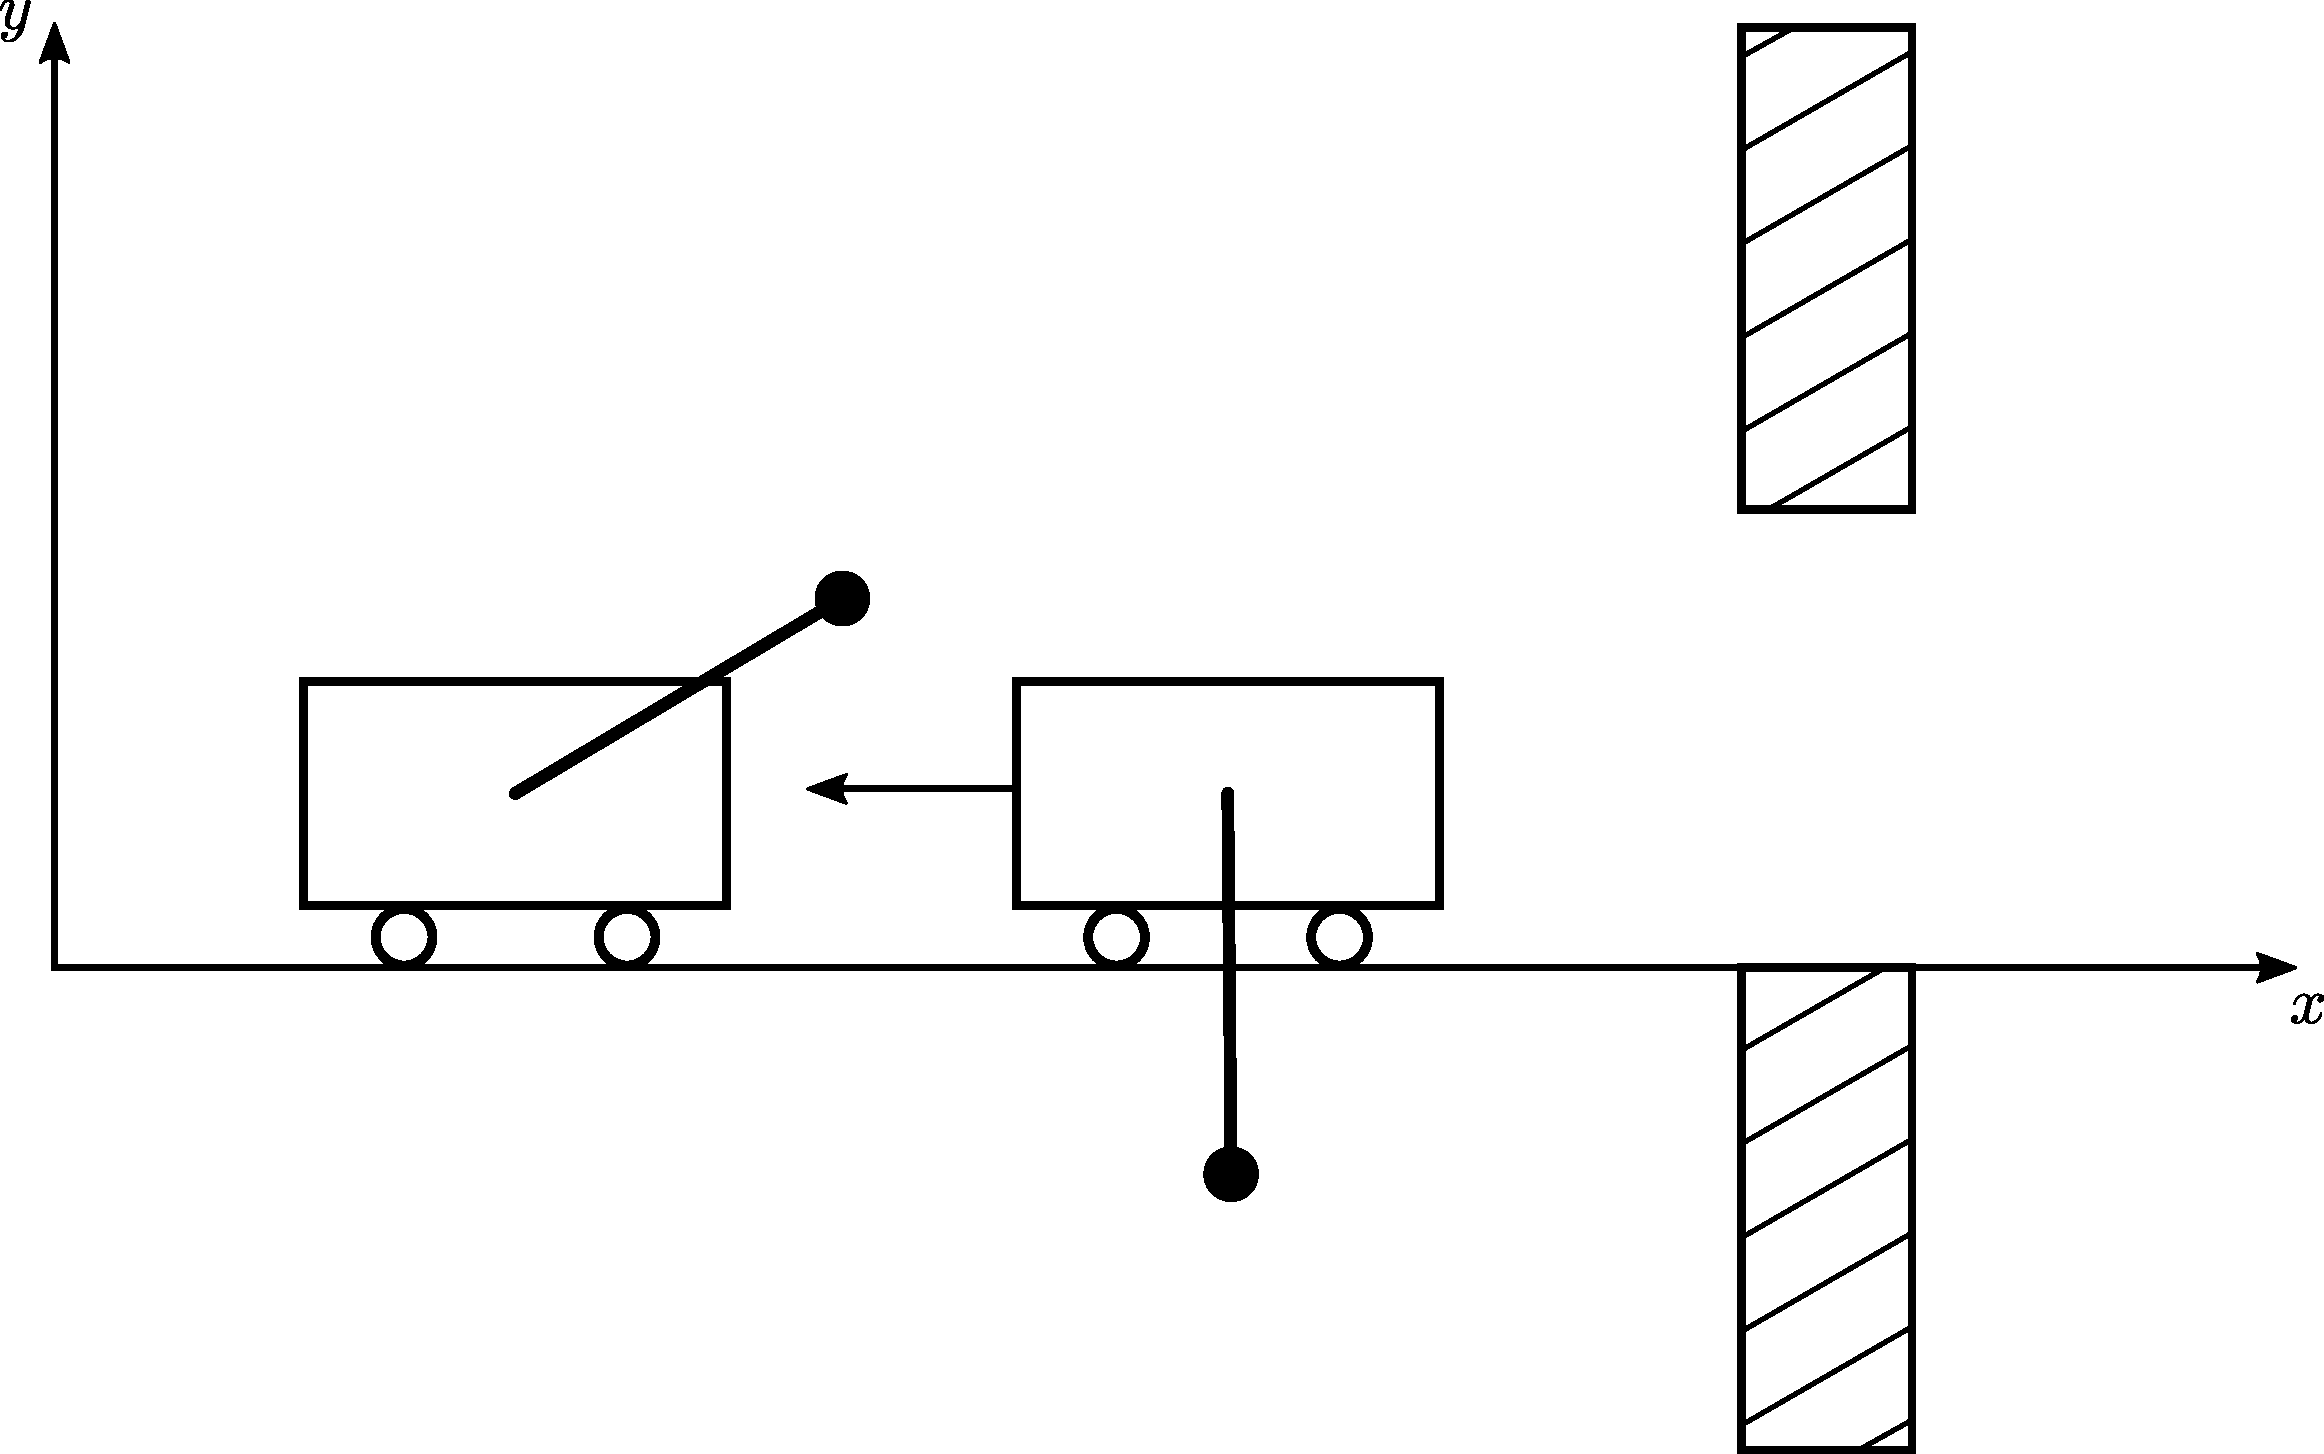
\includegraphics[width=.5\textwidth]{figures/firstTask}
  \caption{The first task is to find a trajectory which raises the pendulum to a position where it is clear of the obstacles in the horizontal direction. Further, to maintain clearance, the angular velocity should hit zero as the target angle is achieved.}
  \label{fig:firstTask}
\end{figure}
%
%Inspecting the phase portrait in \autoref{fig:phasePortrait}\fxnote{update fig ref}, showing the natural theta-dynamics, it is possible to get an idea of how the pendulum moves. The starting position would be the right-most equilibrium of the phase portrait. If this task should be achieved without external force, the pendulum would have to be initialized in the orbit containing the desired final values. However, by exerting a force on the cart it is possible to shift the theta-dynamics. This is further investigated in the next chapter.
%
Assuming that the pendulum was raised above $\frac{\pi}{2}$ while briefly achieving zero angular velocity, the next task would be to maintain zero angular velocity while moving the cart, passing the pendulum through the obstacles, see \autoref{fig:secondTask}.

\begin{figure}[H]
  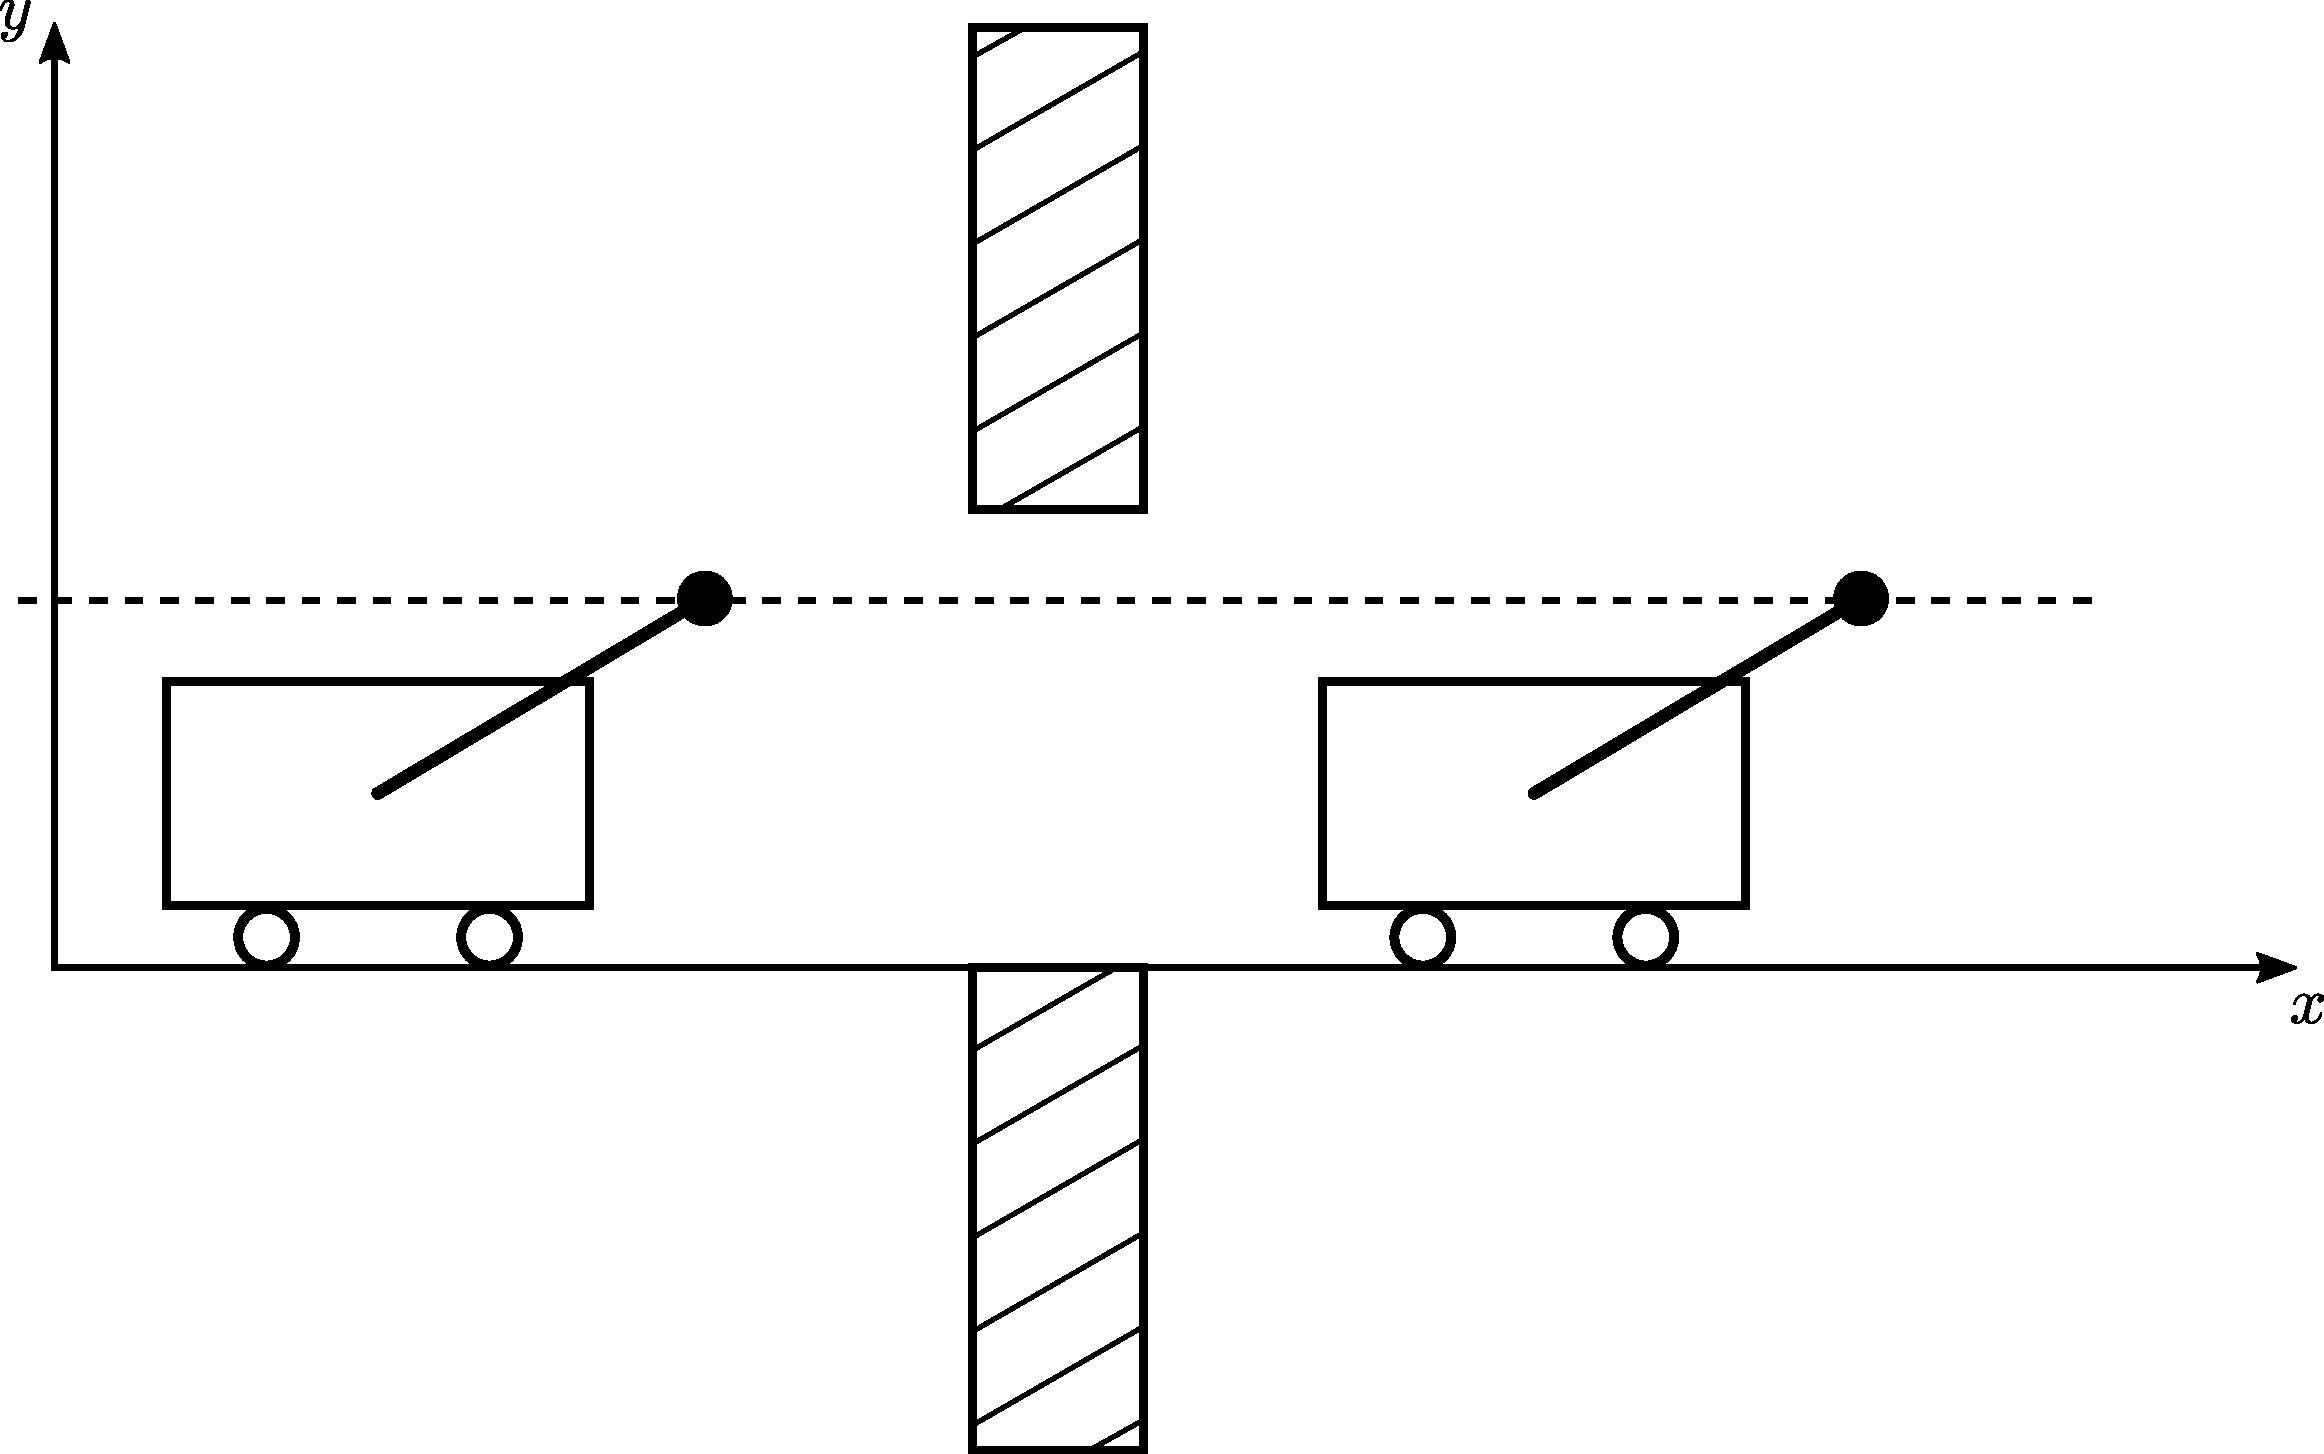
\includegraphics[width=.5\textwidth]{figures/secondTask}
  \caption{The second task is to find a trajectory which keeps the angle and angular velocity at zero as the pendulum is moved with the cart through the obstacles. This can be seen as a virtual constraint where the pendulum mass is constrained to the dotted line.}
  \label{fig:secondTask}
\end{figure}

Ideally this trajectory is a straight horizontal line. This can be seen as a virtual constraint that forces the angle and the angular velocity to stay unchanged. The result will be significantly reduced dynamics, which can be used to directly achieve the desired trajectory.

Finally it is necessary to recover the system on the other side of the obstacles. It is found that this can be achieved, to some extend, by reversing the first trajectory.